\documentclass[12pt]{ctexart}
\usepackage{geometry}
\geometry{a4paper, scale=0.9}
\begin{document}
\begin{verbatim}
    \usepackage{tikz}
    \usetikzlibrary{arrows, backgrounds, ...}
    %坐标绘图,原点位于左下角
    %每条命令后有分号
    %省略单位默认cm

    hello\tikz{\draw (0pt, 0pt)--(30pt, 6pt);}world

    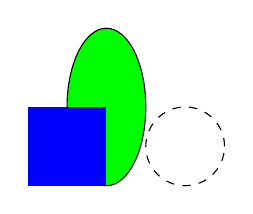
\begin{tikzpicture}
        \draw[style=dashed] (2, 0.5) circle (0.5);
        \draw[fill=green] (1, 1) ellipse (0.5 and 1);
        \fill[blue] (0, 0) rectangle (1, 1);
    \end{tikzpicture}

    %path路径
    \tikz{\path[draw, thick] (1, 1)--(2, 2)--(3, 1)--cycle;}
    \tikz{\path[draw, fill=green!30] (1, 1)--(2, 2)--(3, 1);}
    \tikz{\path[fill=green!30] (1, 1)--(2, 2)--(3, 1);}

    %常用缩写
    \draw = \path[draw]
    \fill = \path[fill]
    \clip = \path[clip]
    \filldraw = \path[fill, draw]
    \shade = \path[shade]

    \tikz\draw (0, 0) arc (45: 135: 1);
    \tikz\draw (0, 0) arc (35: 275: 1 and 0.5);
    \tikz\draw (0, 0) parabola (1, 2);
    \tikz\draw (0, 0) parabola bend (1, 1) (2, 0);

    \begin{tikzpicture}
        \draw[solid] (0, 0)--(0, 3);
        \draw[dashed] (0, 0)--(0, 3);
        \draw[dotted] (0, 0)--(0, 3);
        \draw[loosely dashed] (0, 0)--(0, 3);
        \draw[densely dotted] (0, 0)--(0, 3);
    \end{tikzpicture}

    
\begin{tikzpicture}
        \draw[blue, fill=green] (0, 0) rectangle (2, 1);
        \fill[blue, opacity=0.8] (0, 0) rectangle (1, 2);
    \end{tikzpicture}

    \usetikzlibrary{backgrounds}
    \begin{tikzpicture}[scale=0.8, show rectangle background]
        \draw[fill=blue] (0.5, 0.5)--(1, 1)--(2, 0)--cycle;
    \end{tikzpicture}

    %两种坐标系统 (x, y) 或 (\theta : r)
    %相对位置 +(2pt, 3pt) 或 ++(2pt, 3pt)
    %一个加号不改变当前点,两个加号改变当前点
    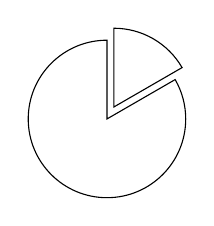
\begin{tikzpicture}
        \draw (0, 0) -- (90: 1cm) arc (90: 390: 1cm) -- cycle;
        \draw (60: 5pt) -- +(30: 1cm) arc (30: 90: 1cm) -- cycle;
    \end{tikzpicture}

    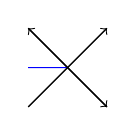
\begin{tikzpicture}
        \draw (0, 0) -- (1, 1);
        \draw (1, 0) -- (0, 1);
        \draw[blue] (0, 0.5) -- (intersection of 0,0--1,1 and 1,0--0,1);
            %交点中的直线不带括号
        \draw[->] (0, 0) -- (1, 1);
        \draw[<->] (1, 0) -- (0, 1);
    \end{tikzpicture}

    \usetikzlibrary{arrows}
    \begin{tikzpicture}
        \draw[thick, ->, >=stealth] (0, 0) -- (1, 1);
        \draw[o-stealth] (1, 0) -- (0, 1);
    \end{tikzpicture}

    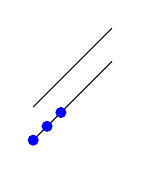
\begin{tikzpicture}
        %坐标变换, shift(.xy)平移, rotate(.)旋转, scale(.xy)缩放, slant(xy)倾斜斜率
        \draw (0, 0) -- (1, 1) [yshift=12pt] (0, 0) -- (1, 1);
        \fill[blue] (0, 0) circle (2pt) %
            [shift={(5pt, 5pt)}] (0, 0) circle (2pt) %
            [shift={(5pt, 5pt)}] (0, 0) circle (2pt);
    \end{tikzpicture}

    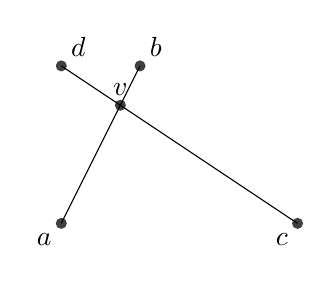
\begin{tikzpicture}
        \coordinate [label=-135:$a$] (a) at (0, 0);
        \coordinate [label=30:$b$] (b) at (1,2);
        \coordinate [label=-135:$c$] (c) at (3, 0);
        \coordinate [label=30:$d$] (d) at (0,2);
        \draw (a) -- (b) (c) -- (d);
        \coordinate [label=90:$v$] (v) at (intersection of a--b and c--d);
        \foreach \p in {a, b, c, d, v} %
            \fill [opacity=0.75] (\p) circle (2pt);
    \end{tikzpicture}

    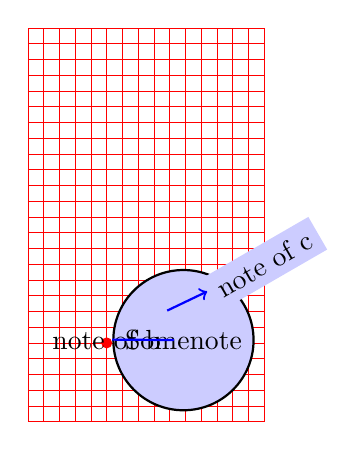
\begin{tikzpicture}[thick, fill=blue!20]
        \draw[step=0.2cm, red, very thin] (0, 0) grid (3, 5);
        \fill[red] (1, 1) circle (2pt);
        \node (a) [above = 1pt, right=2pt] at (1, 1) [draw, fill, circle] {Somenote};
        \node (b) [below=3pt] at (1, 2) [circle] {note of b};
        \node (c) at (3, 2) [fill, rotate=30] {note of c};
        \draw (a) -- (b) [blue, ->] -- (c);
        %more info of node: P70 of "texdoc tikz"
    \end{tikzpicture}   
\end{verbatim}
\end{document}